\section{Introduction}
\label{sec:Intro}

In many prevalent application domains, such as business to business (B2B)~\cite{Lin_B2B}, social networks~\cite{Adar_Managing_2007,Kempe_Maximizing_2003}, and sensor networks~\cite{ZhangSensorNetwork}, graphs serve as powerful models to capture the complex relationships inherent in these applications. 
Most graphs in these applications are uncertain by nature, where each edge carries a degree of uncertainty (probability) representing the probability of its presence in the real world. This uncertainty can be due to various reasons ranging from the use of prediction models to predict the edges (as in social media and B2B networks)  to physical properties that affect the edges' reliabilities (as in sensor and communication networks).  

These uncertain graphs are of significant importance to support various data mining tasks {\eg}, 
understanding  graph structures~\cite{Bollacker_Freebase_2008,Krogan_Global_2006}, social interactions~\cite{Cho_Friendship_2011}, 
information discovery and propagation~\cite{Zhao_Detecting_2014}, advertising and marketing~\cite{Kempe_Maximizing_2003}, among many others.
When compared to sharing the results of data mining, data publishing gives greater flexibility for unlimited analysis,  wider data exploration. However, the publishing of these uncertain graphs might violate participants' privacy.   

\begin{figure}[!htb]
    \subfigure[Social Trust Network]{\label{fig:socialNetwork}
      \begin{minipage}[l]{0.4\columnwidth}
        \centering
        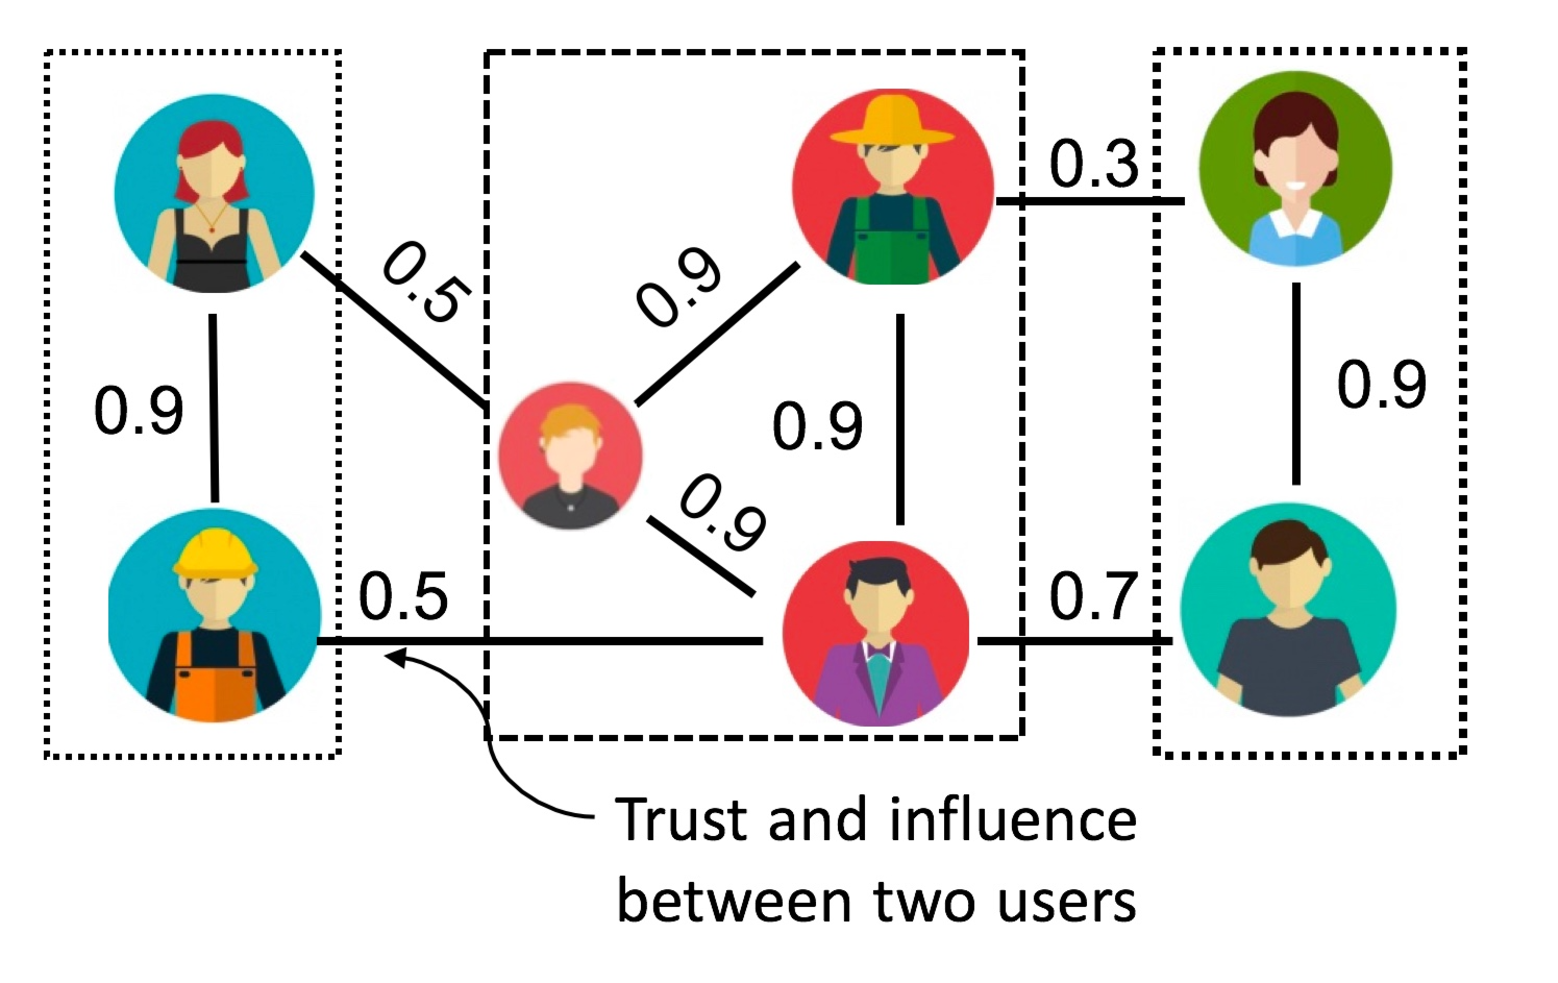
\includegraphics[height=3cm]{ill/SocialNetwork.pdf}
      \end{minipage}
      }
    \subfigure[B2B Network]{\label{fig:b2bNetwork}
      \begin{minipage}[l]{0.4\columnwidth}
        \centering
        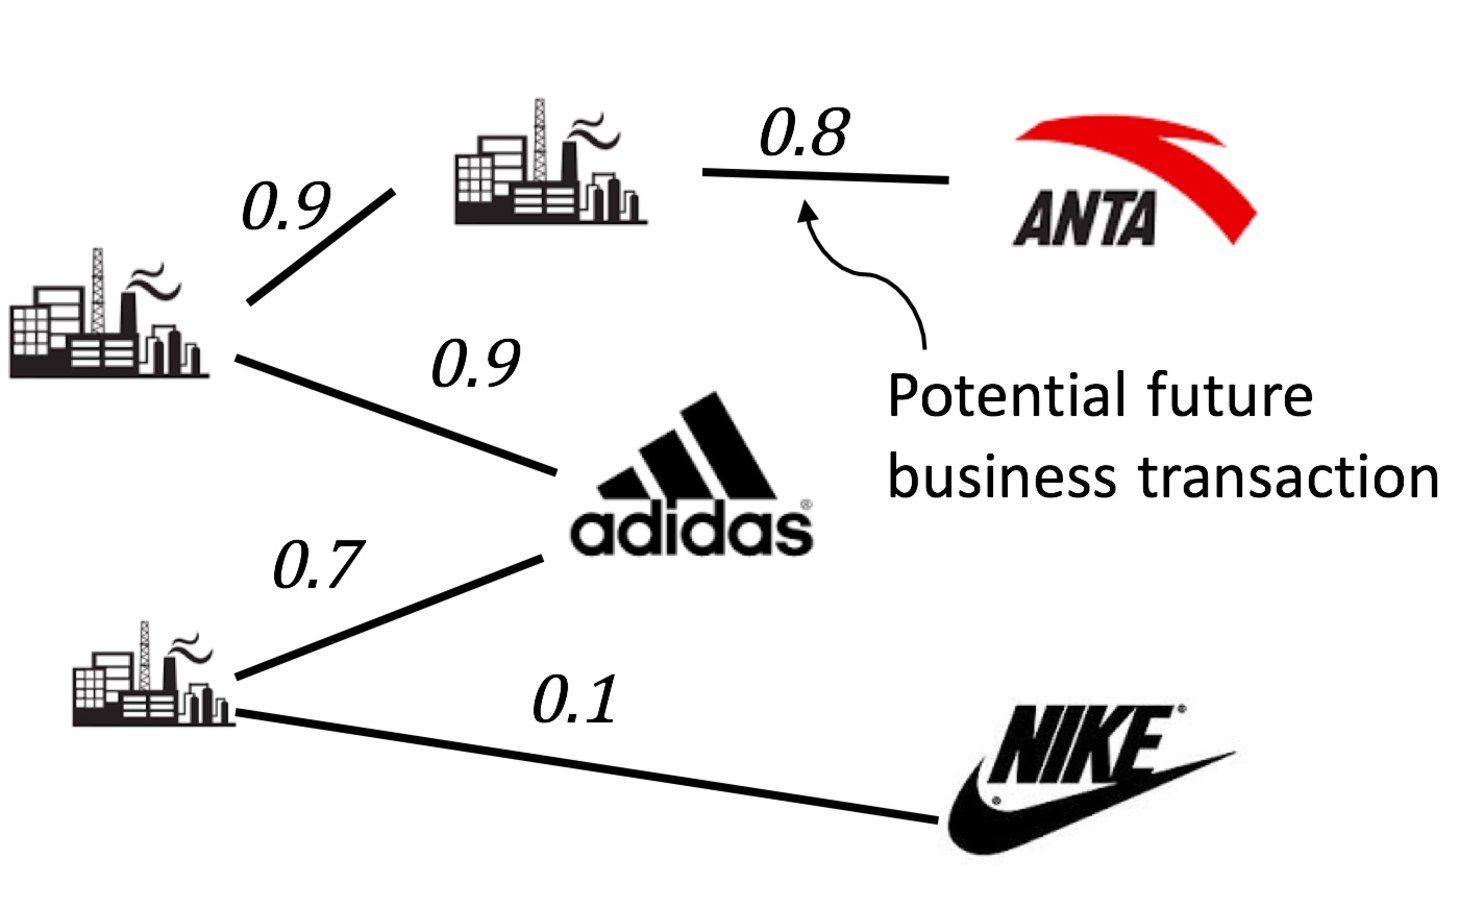
\includegraphics[height=3cm]{ill/B2BNetwork.pdf}
      \end{minipage}
      }
    \vspace{-10pt}
    \caption{Examples of real-world uncertain graphs with privacy concerns.}
    \vspace{-5pt}
\end{figure}


{\textbf{Motivation Scenario I (Social Trust Networks): }}
{\em 
In social networks, the trust and influence relationships among users---which may greatly impact users' behaviors---are usually probabilistic~\cite{Kempe_Maximizing_2003} 
(See Figure~\ref{fig:socialNetwork}). The existence of the trust relationship depends on many factors, such as the area of expertise and emotional connections.
Studying the structure of \emph{real} social trust networks cam produce insights on product promotion, information dissemination. 
However, the release of such uncertain graphs with simple anonymization may cause serious privacy issues.
Equipped with prior knowledge, the attackers can re-identify private and sensitive information, such as the identity of the users and their trustiness relationship, from the released data.
}

\vspace{2mm}
{\textbf{Motivation Scenario II (B2B Networks): }}
{\em  Another example comes from Businesses to Businesses network (See Figure~\ref{fig:b2bNetwork}). In these networks, e.g., ``Alibaba'', nodes represent companies (or business in general) 
while edges represent the trust and the likelihood of future transactions among them~\cite{Lin_B2B}. Such future interactions are probabilistic and obtained by prediction models. The historical transaction releasing is forbidden by legal regulation. 
B2B networks can be analyzed and mined for various applications including advertisement targeting~\cite{Abrahams20132777} and customer segmenting~\cite{alsina2015targeting}. 
Certainly, information about a company's transactions with other companies is considered sensitive data since any leak can be used to infer the company's financial conditions.
}
 
\vspace{2mm}
These scenarios show the immediate need for efficient methods privacy preserving uncertain graph publishing, where sanitation or anonymization is applied to the input uncertain graph before publishing. Despite the number of graph anonymization techniques have been proposed~\cite{Liu_Towards_2008, Boldi_Injecting_2012,  Mittal_Preserving_2013, Bonchi_Identity_2014}, the ignorance of edge uncertainty makes them inefficient for uncertain graph sanitation task. The inefficiency can be due to various reasons ranging from the wrong assumption of privacy attacks to improper utility loss metrics. We face three key challenges in shifting conventional methods to privacy protection on \emph{uncertain graphs}. 

\vspace{2mm}\hspace{-1em}
% \textbf{$\bullet$ Privacy Attacks leveraging Edge Uncertainty:} 
% In Figure \ref{fig:motivation}, we show two instances of released (and {\em ``hopefully anonymized''}) graphs with the same exact topology. 
% In Figure \ref{fig:motivation}(a), the graph is deterministic, while in Figure \ref{fig:motivation}(b), the graph is uncertain with probabilities associated to its edges. 
% The goal of anonymization is to make nodes indistinguishable in spite of external information. 
% We also assume that the adversary has the same knowledge in both cases, i.e., user {\tt Ana} has a degree of $3$ in the original graph. 
% As indicated in the figure, in the case of the deterministic graph, 
% the adversary can \emph{not} re-identify Ana with high confidence since there are two nodes \{{\tt a}, {\tt c}\} each with the matching degree $3$. 
% However, in the uncertain case, the revealed edge uncertainties make the two nodes follow different degree distributions, and thus  
% the adversary has more confidence (around 90\%) that {\tt Ana} maps to Node {\tt a}. 

% This example shows that the release of the associated edge uncertainty increases the potential privacy risk. 
% Therefore, uncertain graph anonymization must take into consideration these edge uncertainties, otherwise, it will fail to protect the privacy correctly.  
% Evidently, ignoring the probabilities altogether and not adding them to the released graph in Figure \ref{fig:motivation}(b) is not a practical solution as it 
% severely destroys  the structure and the utility of the original graph. 


\vspace{2mm}\hspace{-1em}
\textbf{$\bullet$ Appropriate Utility Loss Metric for Uncertain Graphs:} 
Ideally, the anonymized graph should preserve the privacy with the smallest utility loss for further analysis tasks. Thus, it is crucial to understand and model the utility loss of \emph{uncertain graph} being published through well-defined metrics. 
There have been many attempts such as Graph Edit Distance~\cite{Liu_Towards_2008}, Spectrum Discrepancy~\cite{Ying_Randomizing_2008}, Community Reconstruction Error~\cite{Wang2011} and Shortest Path Discrepancy~\cite{Liu_Privacy_2009}.  Most of them heavily tailored towards for deterministic graphs and built on the top of \emph{deterministic} graph concepts. Thus, they are unreasonable when dealing with uncertain graphs. What is the appropriate metric? How is it integrated into anonymization process as replacement of conventional ones? These questions should be carefully addressed when dealing with uncertain graph anonymization. 

\vspace{2mm}\hspace{-1em}
\textbf{$\bullet$ Increased Exponential Complexity of Uncertain Graph Anonymization:}
The problem of $k$-anonymizing a given deterministic graph by as few graph contractions (edge addition, edge deletion, vertex addition and vertex deletion) as possible is shown to be NP-hard~\cite{Hartung_Theory_2015}. Existing techniques usually rely on heuristics to avoid combinatorial
intractability. In uncertain graphs, the problem is even harder since an edge operation is no longer a binary operation (addition or deletion), but there can be infinite probability values that can be assigned to each edge. Therefore, efficient {\em uncertainty-aware} heuristics need to be developed to bring the solution to the realm of feasibility.


%A straightforward approach for anonymizing a given uncertain graph $\mathcal{G}$ which works around ever-mentioned challenges is to combine two existing---but isolated---pieces of work in literature. 
%It anonymizes an uncertain graph in two steps: extract a representative deterministic graph (say $G$) from the input uncertain graph~\cite{Parchas_Gullo_Papadias_Bonchi_2014}, then apply an existing anonymization techniques over $G$ which generates an uncertain graph as the result anonymized version~\cite{Boldi_Injecting_2012,Ying_Randomizing_2008} (referred to as \texttt{Rep-An}). Unfortunately, as we will explain in Section~\ref{sec:repOB}, this approach significantly degrades the utility. 

%\begin{figure}[!t]
%	\centering
%	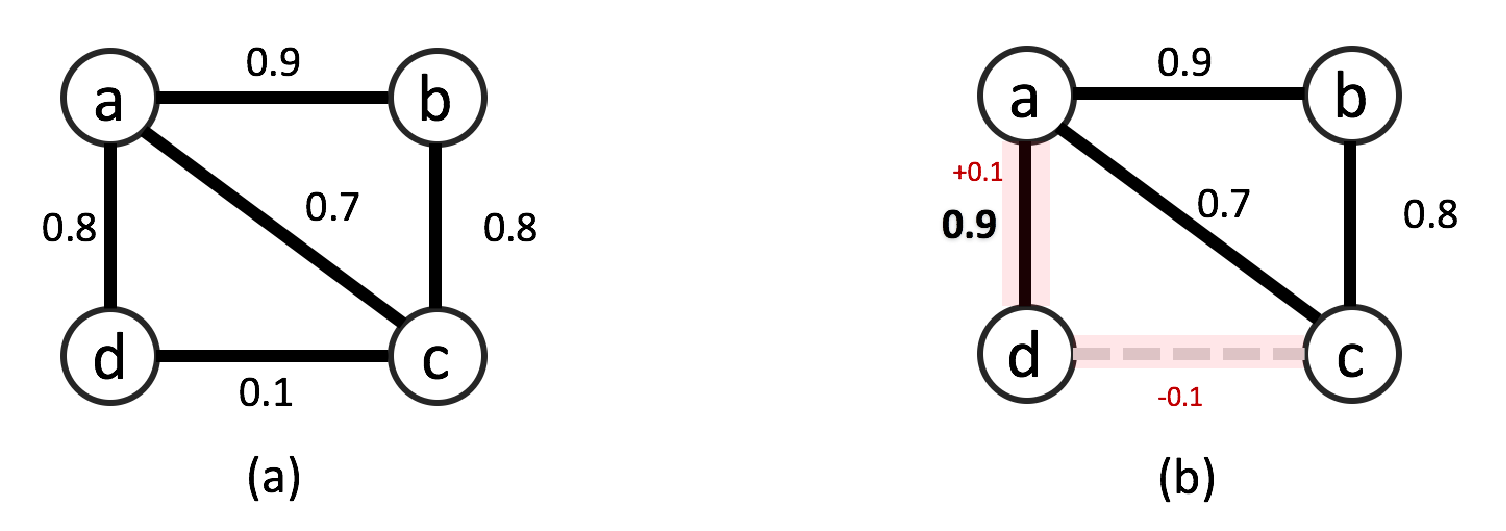
\includegraphics[scale=0.25]{ill/method_ill.eps}
%    \caption{(a) An uncertain graph;(b) a possible anonymization.}
%    \label{fig:method_ill}
%    \vspace{-2em}
%\end{figure}

%******{\todo{You had in the old version a figure (Fig 2). I deleted this one. It does not add much to the paper and not needed.}}*******
\vspace{2mm}


In this paper, we present a principled extension of graph anonymization techniques in the presentence of uncertainty, called \SysName. 
\SysName incorporates edge uncertainties into the core of the  anonymization processing such as evaluations of privacy gain and utility loss. 
In contrast to the classical deterministic graph utility metrics, we propose a new utility metric based on the {\em reliability} measure---which is a core metric in numerous uncertain graph applications~\cite{Asthana_Predicting_2004,Zhao_Detecting_2014,Ghosh_On_2007}. 
The anonymization process need to change the graph structure by modifying the edge probabilities of a subset of the edges, which is an exponential search space. 
Therefore, we propose a ranking algorithm that ranks the edges w.r.t the impact of a change on the graph structure---which we refer to as {\em ``reliability Relevance''}---and 
that ranking will guide the edge selection process. 
Moreover, we propose a theoretically-founded probability-alteration strategy based on the entropy of graph degree sequence, which enables achieving maximum privacy gain for an added amount of 
perturbation. 


% {\todoB{The last sentence does not read well....long chain of dependent words like "max entropy based edge probability perturbation scheme". Needs re-writing...}}

% {\todo{In the last 2 or 3 sentences above: We need a name other than RS....We need to make everything start with \SysName... It can be \SysNameNS-RS....But why "S" in the name? If it is reliability centrality, then should not it be "RC" not "RS". Actually you do not need to introduce the name here..}}

%. Our approach alters the existence probability of the edges of the graph to reach a desired level of identity obfuscation. An example of the proposed PPU method is shown in Figure~\ref{fig:method_ill}. The graph (a) is the original graph that needs to be anonymized; the published graph (b) is a possible anonymization; the anonymization processing involves increment/decrement alterations of existence probability of edges in the uncertain graph.  

%It is very challenging to balance the gain of privacy and the loss of utility when applying alterations over the uncertain graph. 

%To this end, we propose a utility cost metric to capture the connectivity structure change of the uncertain graph. 

%We introduce an efficient algorithm to capture the varying spreading impact of edge probability alteration on different edges--reliability centrality. 
%We leverage these value to perform edge perturbation that sensitive to reliability centrality (referred to as \texttt{RS}). 
%
%The proposed \texttt{RS} scheme favors the perturbation on any edges with slight changes over structural integrity. 
%
%Based on graph entropy model, we propose a max entropy based edge probability perturbation scheme. This is beneficial in the gain of privacy per edge prob alteration.   

In summary, the key contributions of this paper are the following:
% {\todo{Need to go back to these later...}}
\begin{itemize}
\itemsep0em 
\item{Identifying  the new and important problem of uncertain graph anonymization where edge uncertainties need to be seamless 
	integrated into the core of the anonymization process. Otherwise, either the  privacy will not be protected or the  utility will be severely damaged.    
}

\item{Proposing a new utility-loss metric based on the solid connectivity-based graph model under the possible world semantics, namely the {\em reliability discrepancy} (Section \ref{sec:notation}).}

\item{Introducing a theoretically-founded criterion, called {\em reliability relevance}, that encodes the sensitivity of the graph edges and vertices to 
	the possible injected perturbation. The criterion will guide the edges' selection during the anonymization process (Section \ref{sec:tech}).}

\item{Proposing uncertainty-aware heuristics for efficient edge selection and noise injection over the input uncertain graph  to achieve anonymization  
at  a slight cost of reliability  (Section \ref{sec:tech}).}


\item{Building  the \SysName framework that integrates the aforementioned contributions. \SysName is experimentally evaluated using several real-world datasets 
	to evaluate its effectiveness and efficiency. 
	The results demonstrate a significant advantage over the conventional methods that do not directly consider edge uncertainties (Section \ref{sec:exp}).}



%\item{We identify the ineffectiveness of the naive \texttt{Rep-An} approach on preserving the uncertain graph utility for removing uncertainty.}

      
%\item{We conduct experiments over three real-world datasets to compare the effectiveness and efficiency of anonymization approaches. 
%The results demonstrate a significant advantage of our methods over the conventional method which does not directly consider edge uncertainty (Section \ref{sec:exp}).}

\end{itemize}